\documentclass[twoside]{article}
\usepackage[utf8]{inputenc}
\usepackage[brazil]{babel}
%\usepackage[latin1]{inputenc}
\usepackage[sc]{mathpazo} % Use the Palatino font
\usepackage[T1]{fontenc} % Use 8-bit encoding that has 256 glyphs
\linespread{1.05} % Line spacing - Palatino needs more space between lines
\usepackage{microtype} % Slightly tweak font spacing for aesthetics
\usepackage[hmarginratio=1:1,top=32mm,columnsep=20pt]{geometry} % Document margins
\usepackage{multicol} % Used for the two-column layout of the document
\usepackage[hang, small,labelfont=bf,up,textfont=it,up]{caption} % Custom captions under/above floats in tables or figures
\usepackage{booktabs} % Horizontal rules in tables
\usepackage{graphicx}
\usepackage{float} % Required for tables and figures in the multi-column environment - they need to be placed in specific locations with the [H] (e.g. \begin{table}[H])
\usepackage{hyperref} % For hyperlinks in the PDF
\usepackage{lettrine} % The lettrine is the first enlarged letter at the beginning of the text
\usepackage{paralist} % Used for the compactitem environment which makes bullet points with less space between them
\usepackage{abstract} % Allows abstract customization
\renewcommand{\abstractnamefont}{\normalfont\bfseries} % Set the "Abstract" text to bold
\renewcommand{\abstracttextfont}{\normalfont\small\itshape} % Set the abstract itself to small italic text
\usepackage{titlesec} % Allows customization of titles
\renewcommand\thesection{\Roman{section}} % Roman numerals for the sections
\renewcommand\thesubsection{\Roman{subsection}} % Roman numerals for subsections
\titleformat{\section}[block]{\large\scshape\centering}{\thesection.}{1em}{} % Change the look of the section titles
\titleformat{\subsection}[block]{\large}{\thesubsection.}{1em}{} % Change the look of the section titles
\usepackage{fancyhdr} % Headers and footers
\pagestyle{fancy} % All pages have headers and footers
\fancyhead{} % Blank out the default header
\fancyfoot{} % Blank out the default footer
\fancyhead[C]{Um Estudo sobre Possíveis Fatores e suas Relações para o Sucesso de Filmes no Cinema$\bullet$ Dezembro 2014 $\bullet$ } % Custom header text
\fancyfoot[RO,LE]{\thepage} % Custom footer text


%----------------------------------------------------------------------------------------
%	TITLE SECTION
%----------------------------------------------------------------------------------------

\title{\vspace{-15mm}\fontsize{24pt}{10pt}\selectfont\textbf{Um Estudo sobre Possíveis Fatores e suas Relações para o Sucesso de Filmes no Cinema}} % Article title

\author{
\large
\textsc{Yvens Rebouças Serpa}\\[2mm] % Your name
\normalsize Universidade de Fortaleza \\ % Your institution
\normalsize \href{mailto:yvensre@gmail.com}{yvensre@gmail.com} % Your email address
\vspace{-5mm}
}
\date{}

%----------------------------------------------------------------------------------------

\begin{document}

\maketitle % Insert title

\thispagestyle{fancy} % All pages have headers and footers

%----------------------------------------------------------------------------------------
%	ARTICLE CONTENTS
%----------------------------------------------------------------------------------------

\begin{multicols}{2} % Two-column layout throughout the main article text

\section{Introdução}

\lettrine[nindent=0em,lines=3]
A indústria cinematográfica é um dos setores de entretenimento mais populares e lucrativos do mundo. Segundo dados da \textit{Motion Picture Association of America} (MPAA), a receita de bilheteria nos Estados Unidos aproxima-se da cifra de US\$ $9.5$ bilhões no ano de 2006 [1]. No entanto, a produção de um curta ou longa metragem requer altos valores de investimento inicial. Um filme pertencente a uma companhia integrante da MPAA, por exemplo, custa em média US\$ $100.3$ milhões, incluindo os custos de produção, comercialização e \textit{marketing} [1]. Contudo, como toda atividade de empresa, a produção de filmes é uma atividade de risco, tendo em vista a relativa imprevisibilidade da preferência do público.

Este trabalho procura analisar os perfis de diferentes filmes, suas características e avaliações de usuários, para identificar possíveis padrões e informações que possivelmente caracterizam se um filme será um sucesso ou um fracasso. Tais informações minimizariam o risco na produção de filmes e auxiliariam diretores e produtores nesse processo, guiando-os por parâmetros que aumentariam significativamente as chances de sucesso no empreendimento.

A maioria das pesquisas nessa área busca analisar as críticas e \textit{reviews}, classificando-as como positivas ou negativas, para compreender a opinião do público quanto ao filme [2,3,4]. Outra abordagem comum são os sistemas de recomendação que tentam, através das críticas e \textit{reviews} prévias de um determinado usuário, identificar possíveis filmes recomendáveis [5]. Trabalhos com o foco na recepção do público aos filmes são raros e escassos.

Partindo de dados coletados na \textit{Internet Movies Database} (IMDb), nós coletamos diferentes variáveis (gênero, duração, faixa etária, etc.) buscando classificá-los como "Bom", "Regular" ou "Ruim", usando algoritmos de \textit{machine learning}. As classificações foram definidas a partir das avaliações médias dos usuários (\textit{rating} no site. Utilizando árvores de decisão conseguimos uma média de 66\% de acerto, indicando possíveis padrões e variáveis a serem mais profundamente estudadas.

%------------------------------------------------

\section{Trabalhos Relacionados}

Aprendizado de Máquina é uma sub-área da Inteligência Artificial responsável pela modelagem de programas de computador capazes de se desenvolverem automaticamente a partir da experiência [6]. Nesse contexto, diferentes algoritmos foram desenvolvidos ao longo dos anos. Dentre esses algoritmos, podemos citar Árvores de Decisão, Regressão Logística e métodos estatísticos, como Nayve Bayes [6].

Árvores de Decisão são geralmente utilizadas no contexto de avaliação de filmes, na tentativa de identificar padrões e relações entre avaliações prévias de usuários, como apresentado em [3]. Nesse trabalho, esse algoritmo é utilizado para sistemas genéricos de recomendação e, em [2], especificamente para prever o \textit{rating} de um filme de acordo com um histórico de \textit{rating} de cada usuário.

Mais especificamente, em [2], partindo de 9 mil filmes, os autores realizam a previsão de \textit{rating} dos filmes gerando árvores individuais por usuário e métodos colaborativos. As variáveis avaliadas dos filmes foram gênero, atores, diretores e roteristas.

%------------------------------------------------

\section{Solução Proposta}

Esta seção destina-se a explicação da solução proposta.

\subsection{Variáveis Estudadas}

Partindo do trabalho realizado em [2], o qual utiliza as variáveis gênero, atores, diretores e roteristas, propomos mais uma variedade de variáveis a serem analisadas. Primeiramente, utilizamos as variáveis gênero, classificação indicativa (\textit{General}, \textit{Rated}, \textit{Parental Guidance 13}, \textit{Parental Guidance} e \textit{Not Rated}) e duração (Curto, Regular, Longo e Muito Longo). A duração foi classificada a partir do seguinte critério: Curto para abaixo de 88 minutos; Regular para abaixo de 122 minutos; Longo para abaixo de 160 minutos; e Muito Longo para os demais.

Os gêneros foram agrupados nos grupos: Drama (\textit{Drama, Family, Romance, History, Reality-TV, Adult, Biography}); Horror (\textit{Horror, Thriller, Mistery}); Ação (\textit{Action, Adventure, Crime, Sci-Fi, Fantasy, War, Western, Sport}); Comédia (\textit{Comedy}); e Outros.

Também utilizamos as informações de atores e diretores, no entanto, pela diversidade muito grande destes dentro dos dados coletados, decidimos pela utilização de variáveis quanto as suas respectivas premiações. Duas variáveis foram definidas para atores e outras duas para atores, seguindo a mesma lógica: "Existe algum ator/diretor premiado?"; e "Existe algum ator/diretor premiado com Oscar?". Para os atores, utilizamos apenas os três principais do filme, definidos pela própria IMDb.

Os prêmios dos atores e diretores está provavelmente relacionada ao sucesso de seus filmes, isto porque, tendo em vista o sucesso em empreendimentos passados, é mais provável que novos empreendimentos sejam também bem sucedidos.

A partir das \textit{tags} definidas pelos usuários e responsáveis pelo IMDb, realizamos a coleta das 200 \textit{tags} principais de cada um dos filmes e realizamos um agrupamento das mais recorrentes em diferentes categorias. Dessa forma, adicionamos uma variável \textit{booleana} para cada um dos agrupamentos de \textit{tags} gerado. Acreditamos que estas variáveis representam temas e elementos importantes na narrativa que podem estar diretamente relacionadas ao sucesso dos filmes. No total são 17 variáveis, a saber:
\\
\begin{compactitem}
\item É violento?;
\item É sangrento?;
\item É sequência de algum filme?;
\item É baseado em livro?;
\item É independente?;
\item Possui cenas de sexo?;
\item Possui cenas de nudez?;
\item Possui armas de fogo?;
\item Possui cenas de \textit{flashback}?;
\item Possui final surpreendente?;
\item Possui tecnologia atual?;
\item Possui efeitos de câmera?
\item Sobre relacionamentos?;
\item Sobre drama humano?;
\item Sobre cidades ou natureza?;
\item Sobre famílias?;
\item Foi escrito pelo diretor?; \\
\end{compactitem}

Por fim, para a classificação do filme utilizamos a média de notas da IMDb e agrupamos em três categorias: Ruim, Regular e Bom. Para tal, seguimos a seguinte regra: Ruim para abaixo de 5.0; Regular para abaixo de 7.0; e Bom para os demais.

\subsection{Coleta de Dados}
Os dados foram coletados utilizando um \textit{crawler web}, lendo os arquivos HTML das páginas da IMDb, analisando os códigos e identificando as informações. Os filmes são todos do período de 2003 a 2013. Cerca de 3000 filmes, bem distribuídos entre as três categorias, foram analisados. Além disso, os dados apresentaram boa distribuição das demais variáveis.

\begin{figure}[H]
\centering
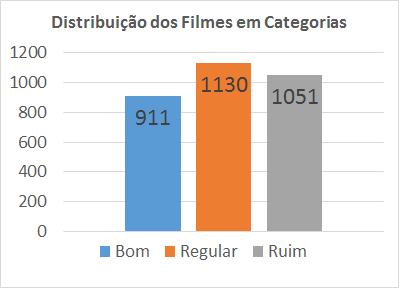
\includegraphics[width=7cm]{grafico_rating.png}
\caption{Distribuição dos Filmes em Categorias}
\label{Rotulo}
\end{figure}

\begin{table}[H]
\caption{Filmes por Categoria}
\centering
\begin{tabular}{ll}
Categoria & Quantidade \\
\midrule
Ruim & $1051$ \\
Regular & $1130$ \\
Bom & $911$ \\
\bottomrule
\end{tabular}
\end{table}

%------------------------------------------------

\section{Resultados da Avaliação}

Testes foram realizados utilizando a plataforma WEKA, executando os algoritmos de Árvore de Decisão (J48), Regressão Logística (Logistic), Nayve Bayes (NayveBayesSimple), K-NN (IBk) e Ensembles (Bagging) . O método de validação utilizado o \textit{Cross-validation} com 10 iterações. Os resultados para estes algoritmos estão presentes na tabela 2 a seguir:

\begin{table}[H]
\caption{Resultado dos Algoritmos}
\centering
\begin{tabular}{l|ll}
Algoritmo & Acerto (\%) & Acerto "Bom"\\
\midrule
J48 & $66.8823$ & 338/911\\
Logistic & $66.7529$ & 377/911\\
Nayve Bayes & $59.7025$ & 164/911\\
IBk & $61.837$ & 320/911\\
Bagging & $66.8823$ & 371/911\\
\bottomrule
\end{tabular}
\end{table}

\subsection{Análise dos Resultados}

Inicialmente, os piores resultados foram apresentados pelo algoritmo estatístico \textit{Nayve Bayes}, o qual aplica métodos de probabilidade assumindo forte independência entre as variáveis analisadas. Essa suposição está claramente equivocada, visto que algumas variáveis estudadas são obrigatoriamente dependentes, como a premiação de um diretor e se este possui algum Oscar em sua carreira, por exemplo.

Em seguida, temos os algoritmos de Regressão Logística e de Árvore de Decisão com resultados bastante próximos, no entanto, o método de Regressão Logística apresenta uma maior quantidade de acertos para a classificação de "Bom" filme, em relação à Árvore de Decisão. Podemos verificar os falsos negativos na tabela 3.

\begin{table}[H]
\caption{Matriz de Confusão - "Bom"}
\centering
\begin{tabular}{l|lll}
Algoritmo & Ruim & Regular & Bom\\
\midrule
J48 & 313/911 & 260/911 & 338/911\\
Logistic & 275/911 & 259/911 & 377/911\\
Nayve Bayes & 411/911 & 336/911 & 164/911\\
IBk & 289/911 & 302/911 & 320/911\\
Bagging & 269/911 & 271/911 & 371/911\\
\bottomrule
\end{tabular}
\end{table}

A grande quantidade de falsos negativos não se repete para as categorias "Ruim" e "Regular", o que indica o ponto de dificuldade dos algoritmos. Além disso, poucos filmes destas classificações são erroneamente classificados como "Bom".

O resultado para o algoritmo de \textit{Ensembles} utilizado, \textit{Bagging}, mostrou que não há grande variação entre as amostras, de forma a produzir diferentes modelos para diferentes grupos de amostras. Dessa forma, o resultado do algoritmo foi muito próximo (percentualmente igual) à árvore de decisão. 

\subsection{Árvore de Decisão}

Embora os resultados para a árvore de decisão não sejam os melhores, a análise de sua estrutura pode relevar padrões e relações entre as variáveis ainda não percebidos pelos pesquisados.

A árvore gerada para os testes possui tamanho igual a 196 e 114 folhas.

O primeiro nó analisado pela estrutura é se o diretor é premiado ou não. Caso ele não seja premiado, existe apenas um caminho na árvore que leva a um possível filme "Bom", enquanto todos os outros preveem que o mesmo será "Regular" ou "Ruim". Esse primeiro ponto leva a questionar a avaliação dos usuários quanto a filmes independentes ou novos no cenário cinematográfico mundial, avaliando novos diretores com notas piores.

\begin{figure}[H]
\centering

\includegraphics[width=7cm]{cloud.jpg}
\caption{Cloud Atlas (2012)}
\label{Rotulo}
\end{figure} 

O próximo nó analisa se o filme possui atores premiados ou não. Nesse ponto também identificamos uma forte tendência a prevê a classificação como "Regular" ou "Ruim" na ausência de atores premiados no elenco do filme. Uma exceção notável é a situação "Diretor premiado; Atores não premiados; Sem Final Surpreendente; Sem Cenas de Nudez; Escrito Pelo Diretor", na qual o classificador indica um potencial filme "Bom", com 96 instâncias positivas e 23 negativas.

Após a análise da premiação dos atores, a duração dos filmes é analisada. Nesse ponto, todos os filmes classificados como "Muito Longos", isto é, acima de 160 minutos, são classificados como "Bom", sem instâncias negativas. Provavelmente, esse é o caso de mega produções como \textit{Cloud Atlas} (2012), Figura 2, ou \textit{Avatar} (2009).

Em uma análise geral, a maioria dos ramos da árvore com as características relacionadas à sexo ou violência não preveem filmes do tipo "Bom", o que vai de encontro à afirmação popular de que estes são temas que vendem. Salvo casos como filmes do tipo "Longo", que não sejam sequência, não escritos por direito, não independentes e sangrentos, com 58 instâncias positivas de "Bom". Provavelmente, esse é o caso de filmes mais adultos com temática de guerra, como \textit{Zero Dark Thirty} (2012), Figura 3.

\begin{figure}[H]
\centering

\includegraphics[width=7cm]{zero.jpg}
\caption{Zero Dark Thirty (2012)}
\label{Rotulo}
\end{figure} 


Com relação ao gênero, para filmes com duração Regular, isto é, até 122 minutos, os gêneros de Horror, Ação e Comédia são massivamente e diretamente considerados como "Regular", com, respectivamente, 67, 276 e 283 instâncias positivas contra 16, 61 e 84 instâncias negativas. Já os filmes de Drama passam por uma análise mais detalhada.

O algoritmo foi executado com poda, o que permitiu identificar a ausência de relevância nas variáveis relativas ao oscar de ator ou diretor e na \textit{tag} "sobre cidades ou natureza".

\section{Conclusão e Trabalhos Futuros}

Neste trabalho analisados diferentes variáveis presentes em 3000 filmes divididos em 3 categorias de acordo com o \textit{rating} dos usuários e administradores da IMDb. A partir dos dados coletados, diferentes algoritmos de \textit{machine learning} foram aplicados e comparados.

Com resultados ainda tímidos, a Árvore de Decisão apresentou a maior taxa de acerto e possibilitou a análise da relação das diferentes variáveis estudadas. Mais ainda, permitiu a visualização das variáveis mais relevantes no contexto e, através da poda, daquelas sem relevância.

A análise das matrizes de confusão evidenciaram a dificuldade maior dos algoritmos na classificação de filmes na categoria "Bom", o que instiga em mais pesquisas a serem realizadas na área. Concluímos a partir disso de que, diferente de filmes ruins ou medianos, os quais apresentam pontos fixos de falha e rejeição do público, como ausência de atores ou diretores premiados, um filme bom é ainda bastante imprevisível. Algumas sugestões, como mega produções cinematográficas podem ser a resposta para o problema, mas ainda representam um pequeno conjunto de instâncias e apresentam maior risco de produção, devido ao alto valor de investimento financeiro inicial.

No entanto, os testes realizados baseiam-se somente na classificação da IMDb, o que não necessariamente representa a opinião geral, estando sujeita a votações de não especialistas e em amostragem irregulares, isto é, alguns filmes possuírem nota média alta devido à baixa quantidade de votos, enquanto outros filmes possuem notas mais baixas devida à massiva quantidade de votos. O ideal seria gerar uma classificação multicritério utilizando dados de diferentes sites e ponderando as médias de acordo com a quantidade de votos.

%----------------------------------------------------------------------------------------
%	REFERENCE LIST
%----------------------------------------------------------------------------------------

\begin{thebibliography}{9}


\bibitem{cinema_livro}
Alessandra Meleiro. 2007. "Cinema no Mundo, V.4 - Estados Unidos (1 ed.)." Escritura, Inc., São Paulo, SP, Brasil.

\bibitem{artigo2}
Marovic, Mladen, et al. "Automatic movie ratings prediction using machine learning." MIPRO, 2011 Proceedings of the 34th International Convention. IEEE, 2011.

\bibitem{artigo3}
Bobadilla, J. E. S. U. S., Francisco Serradilla, and Antonio Hernando. "Collaborative filtering adapted to recommender systems of e-learning." Knowledge-Based Systems 22.4 (2009): 261-265.

\bibitem{artigo4}
Chaovalit, Pimwadee, and Lina Zhou. "Movie review mining: A comparison between supervised and unsupervised classification approaches." System Sciences, 2005. HICSS'05. Proceedings of the 38th Annual Hawaii International Conference on. IEEE, 2005.

\bibitem{artigo1}
 Gershman, Amir, et al. "A Decision Tree Based Recommender System."
 
\bibitem{ml_livro}
Thomas M. Mitchell. 1997. "Machine Learning (1 ed.)." McGraw-Hill, Inc., New York, NY, USA.

\end{thebibliography}
%----------------------------------------------------------------------------------------

\end{multicols}

\end{document}
